\clearpage
\sffamily
{\bfseries\color[rgb]{0.4,0.4,0.4}
Part B: Goal-Kick from Moving Ball}
\phantomsection
\addcontentsline{toc}{subsection}{Part B: Goal-Kick from Moving Ball}


\bigskip

\added{The goal of the goal-kick from a moving ball challenge is to kick a moving ball
into the goal. Results of the technical challenge are based on a batch of three runs.}

\bigskip

\added{{\bfseries Run Setup}}

\smallskip

\begin{figure}[h]
\begin{center}
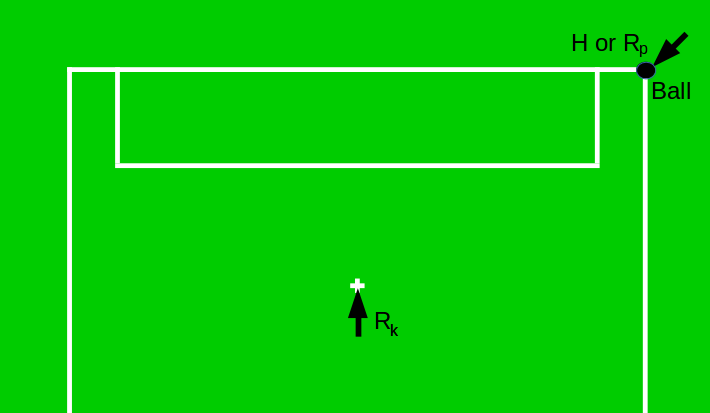
\includegraphics[width=0.6\textwidth]{img/tc_dynamic_kick.png}
\caption{\label{fig:tc_dynamic_kick}Setup for the moving ball challenge.}
\end{center}
\end{figure}

\added{The initial setup of a run is presented in Fig.~\ref{fig:tc_dynamic_kick},
procedure is as follows:}


\begin{enumerate}
\item \added{The ball is placed on one corner of the field as chosen by the team taking the
technical challenge.}
\item \added{The robot $R_K$ is placed on the penalty mark.}
\item \added{The pass of the ball may either be performed by a human member from the
team $H$ or another robot, $R_P$. If the pass is performed by a robot, the team
may place $R_P$ after the referee has placed the ball. $R_p$ can be placed
anywhere on the field, not directly touching the ball.}
\item \added{The referee blows the whistle to start the trial.}
\item \added{Teams may start the robot $R_P$ manually by pressing a button when the
trial starts. But $R_K$ must not be touched after the referee blew the whistle.}
\item \added{A chronometer is started when $R_P$ or $H$ kicks the ball.}
\end{enumerate}

\added{{\bfseries Run evaluation}}

\smallskip

\added{The chronometer is stopped when the trial ends. The causes for trial ends and
the possible results are as following:}
\begin{itemize}
\item \added{\textit{Failure}}
  \begin{itemize}
    \item \added{The ball has been touched twice by $R_P$, $H$ or $R_K$.}
    \item \added{$R_k$ attempted to kick but failed to touch the ball.}
    \item \added{The ball was kicked by $R_k$ but leaves the field without scoring a goal.}
  \end{itemize}
\item \added{\textit{Retake}}
  \begin{itemize}
    \item \added{The ball stops before $R_k$ attempted to kick.}
    \item \added{The ball \emph{bounced} on $R_k$ rather than being kicked.}
  \end{itemize}
\item \added{\textit{Partial success}}
  \begin{itemize}
    \item \added{Ball was kicked by $R_k$ but stopped rolling inside of the field.}
  \end{itemize}
\item \added{\textit{Success}}
  \begin{itemize}
    \item \added{Ball was kicked by $R_k$ and a goal was scored.}
  \end{itemize}
\end{itemize}

\added{{\bfseries Trials and ranking}}

\added{A trial consists of three different runs, each run ending with a \textit{Retake}
is restarted and do not count. A trial is considered as successful if at least 2
runs from the batch resulted in \textit{Success}. A trial is considered as
partially successful if at least 2 runs resulted in \textit{Success} or \textit{Partial success}.}

\added{The teams are ranked according to the following criteria on their best batch:}
\begin{enumerate}
\item \added{Number of \textit{Success} where the pass of the ball was executed by a robot}
\item \added{Number of \textit{Success} where the pass of the ball was executed by a human}
\item \added{Number of \textit{Partial success} where the pass of the ball was executed by a robot}
\item \added{Number of \textit{Partial success} where the pass of the ball was executed by a human}
\item \added{Average time for \textit{Success} runs, from first touch by $R_p$ or $H$ until goal is scored}
\item \added{Average shortest distance to the goal line for \textit{Partial success} runs}
\end{enumerate}


\removed{
The referee places the ball randomly on one corner of the goal area located on
the goal line. The robot $R_K$ is placed on the penalty mark. The pass of the
ball may either be performed by a human member from the team $H$ or another
robot, $R_P$. If the pass is performed by a robot, the team may place $R_P$
after the referee has placed the ball anywhere on the field not directly
touching the ball. The referee blows the whistle to start the trial. Teams may
start the robot $R_P$ manually by pressing a button when the trial starts.  }

\removed{
After the ball has been kicked by $R_P$ or the human, $R_K$ must
make contact with it before the ball comes to a stop, otherwise the trial is
unsuccessful. The trial is also unsuccessful if the ball leaves the field, $R_K$
touched the ball without the ball moving, or after one minute has elapsed since
the start of the trial. If after the ball contact the ball enters the goal, the
trial is successful and the time is stopped at the moment the ball passed the
goal line. Otherwise the trial is partially successful. Teams are first ranked
by the time for fully successful trials and then by the shortest distance
between the ball and the goal for partially successful trials.
}
